% answers.tex —— 2008 年·春季上海卷 · 参考答案与详细解析片段
% 由 tools/generate_projects.py 依来源总账自 2008/2008_数学真题_春季上海_试题.md + 2008/2008_数学真题_春季上海_解析正文.md + 2008/2008_数学真题_春季上海_答案要点.md 生成，勿手改（改源 MD 后重跑）


\begin{gktip}
下列过程以独立盲解为底稿，依据固定题面推导；副本第 3–4 页只作参考答案对照，不认证答案的发布归属或官方性。Q8 的两种方向分别保留，卷级答案记 U。
\end{gktip}

\begin{answer}
\gksolhead{1}{}

\textbf{题目}（4 分）：

\Needspace{5\baselineskip}
已知集合
\nopagebreak[4]
\[
A=\{x\mid x<-1\text{ 或 }2\le x<3\},\qquad B=\{x\mid -2\le x<4\},
\]
则 \(A\cup B=\underline{\qquad\qquad}\)。

\Needspace{4\baselineskip}
\textbf{解析}

由 $B=[-2,4)$，集合 $A$ 中的区间 $[2,3)$ 已包含在 $B$ 内，而 $A$ 还含所有 $x<-1$。因此 $A\cup B=(-\infty,4)$。

\gkanswer{答案：$(-\infty,4)$}

\end{answer}
\begin{answer}
\gksolhead{2}{}

\textbf{题目}（4 分）：

\Needspace{5\baselineskip}
计算
\nopagebreak[4]
\[
\lim_{n\to\infty}\frac{3^n+1}{3^{n+1}+2^n}=\underline{\qquad\qquad}。
\]

\Needspace{4\baselineskip}
\textbf{解析}

\Needspace{5\baselineskip}
分子分母同除以 $3^{n+1}$，得
\nopagebreak[4]
\[
\frac{3^n+1}{3^{n+1}+2^n}
=\frac{\frac13+3^{-(n+1)}}{1+(2/3)^n}\longrightarrow\frac13.
\]

\gkanswer{答案：$\dfrac13$}

\end{answer}
\begin{answer}
\gksolhead{3}{}

\textbf{题目}（4 分）：

\Needspace{5\baselineskip}
函数
\nopagebreak[4]
\[
f(x)=\frac{\sqrt{-x^2+x+6}}{x-1}
\]
的定义域是 \(\underline{\qquad\qquad}\)。

\Needspace{4\baselineskip}
\textbf{解析}

根号内须非负：$-x^2+x+6\ge0$，即 $(3-x)(x+2)\ge0$，所以 $-2\le x\le3$。分母还要求 $x\ne1$，定义域为 $[-2,1)\cup(1,3]$。

\gkanswer{答案：$[-2,1)\cup(1,3]$}

\end{answer}
\begin{answer}
\gksolhead{4}{}

\textbf{题目}（4 分）：

\Needspace{5\baselineskip}
方程
\nopagebreak[4]
\[
2\cos\left(x-\frac\pi4\right)=1
\]
在区间 \((0,\pi)\) 内的解是 \(\underline{\qquad\qquad}\)。

\Needspace{4\baselineskip}
\textbf{解析}

令 $t=x-\pi/4$。方程化为 $\cos t=1/2$，故 $t=\pm\pi/3+2k\pi$。结合 $0<x<\pi$，唯一解为 $x=7\pi/12$。

\gkanswer{答案：$\dfrac{7\pi}{12}$}

\end{answer}
\begin{answer}
\gksolhead{5}{}

\textbf{题目}（4 分）：

已知数列 \(\{a_n\}\) 是公差不为零的等差数列，\(a_1=1\)。若 \(a_1、a_2、a_5\) 成等比数列，则 \(a_n=\underline{\qquad\qquad}\)。

\Needspace{4\baselineskip}
\textbf{解析}

设公差为 $d\ne0$，则 $a_2=1+d$、$a_5=1+4d$。三数成等比给出 $(1+d)^2=1+4d$，即 $d(d-2)=0$；因 $d\ne0$，故 $d=2$，$a_n=1+2(n-1)=2n-1$。

\gkanswer{答案：$a_n=2n-1$}

\end{answer}
\begin{answer}
\gksolhead{6}{}

\textbf{题目}（4 分）：

\Needspace{5\baselineskip}
化简
\nopagebreak[4]
\[
\cos\left(\frac\pi3+\alpha\right)+\sin\left(\frac\pi6+\alpha\right)=\underline{\qquad\qquad}。
\]

\Needspace{4\baselineskip}
\textbf{解析}

\Needspace{5\baselineskip}
用和角公式：
\nopagebreak[4]
\[
\cos\left(\frac\pi3+\alpha\right)+\sin\left(\frac\pi6+\alpha\right)
=\frac12\cos\alpha-\frac{\sqrt3}{2}\sin\alpha
+\frac12\cos\alpha+\frac{\sqrt3}{2}\sin\alpha=\cos\alpha.
\]

\gkanswer{答案：$\cos\alpha$}

\end{answer}
\begin{answer}
\gksolhead{7}{}

\textbf{题目}（4 分）：

\Needspace{5\baselineskip}
已知 \(P\) 是双曲线
\nopagebreak[4]
\[
\frac{x^2}{a^2}-\frac{y^2}{9}=1
\]
右支上的一点，双曲线的一条渐近线方程为 \(3x-y=0\)。设 \(F_1、F_2\) 分别为双曲线的左、右焦点。若 \(|PF_2|=3\)，则 \(|PF_1|=\underline{\qquad\qquad}\)。

\Needspace{4\baselineskip}
\textbf{解析}

双曲线的渐近线斜率为 $3/ a$，与 $3x-y=0$ 比较得 $a=1$；半实轴为 $3$，焦半距 $c=\sqrt{1+9}=\sqrt{10}$。右支上点到两焦点的距离差为 $2a=2$，即 $|PF_1|-|PF_2|=2$，因此 $|PF_1|=5$。

\gkanswer{答案：$5$}

\end{answer}
\begin{answer}
\gksolhead{8}{}

\textbf{题目}（4 分）：

已知一个凹多面体共有 9 个面，所有棱长均为 1，其平面展开图如图 1 所示，则该凹多面体的体积 \(V=\underline{\qquad\qquad}\)。
\nopagebreak[4]
\begin{center}% Q8：固定副本中的展开图拓扑；所有小面边长均为 1。
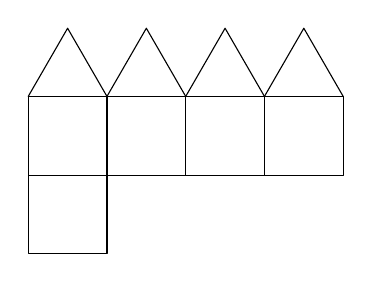
\begin{tikzpicture}[line cap=round,line join=round]
  % 四个侧方形依次相连，底方面连接在最左侧方形下边。
  \draw (0,0) rectangle (1,1);
  \draw (1,0) rectangle (2,1);
  \draw (2,0) rectangle (3,1);
  \draw (3,0) rectangle (4,1);
  \draw (0,-1) rectangle (1,0);
  % 四个等边三角形分别接在侧方形上边。
  \draw (0,1)--(0.5,1.866)--(1,1);
  \draw (1,1)--(1.5,1.866)--(2,1);
  \draw (2,1)--(2.5,1.866)--(3,1);
  \draw (3,1)--(3.5,1.866)--(4,1);
\end{tikzpicture}
\end{center}
\nopagebreak[4]
\Needspace{4\baselineskip}
\textbf{解析}

\Needspace{5\baselineskip}
\textbf{状态待核（U）}。题面称该多面体为“凹多面体”，展开图含一个边长为 $1$ 的方形底面和四个边长为 $1$ 的等边三角形顶面。按凹形折叠，四个三角形形成向内凹入的方锥腔。腔体底面积为 $1$；顶点至底面的高为
\nopagebreak[4]
\[
\sqrt{1-\left(\frac{\sqrt2}{2}\right)^2}=\frac1{\sqrt2}.
\]
外部方形柱体积为 $1$，凹腔体积为 $\frac13\cdot1\cdot\frac1{\sqrt2}=\frac{\sqrt2}{6}$，故按题面文字所得体积为 $1-\frac{\sqrt2}{6}$。固定副本答案页印载 $1+\frac{\sqrt2}{6}$，与“凹”字方向不符；没有同版勘误或更可靠版本前，不把该印载值用于替换题面条件。

\gkanswer{答案：U（按题面文字计算为 $1-\dfrac{\sqrt2}{6}$；固定副本答案页印载 $1+\dfrac{\sqrt2}{6}$）}

\end{answer}
\begin{answer}
\gksolhead{9}{}

\textbf{题目}（4 分）：

\Needspace{5\baselineskip}
已知无穷数列 \(\{a_n\}\) 前 \(n\) 项和
\nopagebreak[4]
\[
S_n=\frac13a_n-1,
\]
则数列 \(\{a_n\}\) 的各项和为 \(\underline{\qquad\qquad}\)。

\Needspace{4\baselineskip}
\textbf{解析}

\Needspace{5\baselineskip}
由 $S_1=a_1=\frac13a_1-1$ 得 $a_1=-\frac32$。对 $n\ge2$，用 $a_n=S_n-S_{n-1}$ 及题设关系可得 $2a_n=-a_{n-1}$，所以数列公比为 $-1/2$，无穷和为
\nopagebreak[4]
\[
\frac{a_1}{1-(-1/2)}=-1.
\]

\gkanswer{答案：$-1$}

\end{answer}
\begin{answer}
\gksolhead{10}{}

\textbf{题目}（4 分）：

古代“五行”学说认为：“物质分金、木、水、火五种属性，金克木，木克土，土克水，水克火，火克金。”将五种不同属性的物质任意排成一列，设事件 \(A\) 表示“排列中属性相克的两种物质不相邻”，则事件 \(A\) 出现的概率是 \(\underline{\qquad\qquad}\)（结果用数值表示）。本题文字跨 PDF 第 1 页双栏。

\Needspace{4\baselineskip}
\textbf{解析}

五行相克关系形成一个 5-cycle。允许相邻的关系图是其补图，也为 5-cycle。在此图上取一条包含全部五个顶点的排列路径，必须删去环中的一条边；有 5 种删边方式，每种有两个方向，共 10 种合法排列。全部排列有 $5!=120$ 种，概率为 $10/120=1/12$。

\gkanswer{答案：$\dfrac1{12}$}

\end{answer}
\begin{answer}
\gksolhead{11}{}

\textbf{题目}（4 分）：

\Needspace{5\baselineskip}
已知 \(a_1,a_2,\ldots,a_n；\ b_1,b_2,\ldots,b_n\)（\(n\) 是正整数），令
\nopagebreak[4]
\[
L_1=b_1+b_2+\cdots+b_n,\quad L_2=b_2+b_3+\cdots+b_n,\quad
L_3=b_3+\cdots+b_n,\quad\ldots,\quad L_n=b_n。
\]
\Needspace{5\baselineskip}
某人用图 2 分析得到恒等式
\nopagebreak[4]
\[
a_1b_1+a_2b_2+\cdots+a_nb_n
=a_1L_1+c_2L_2+c_3L_3+\cdots+c_kL_k+\cdots+c_nL_n，
\]
则 \(c_k=\underline{\qquad\qquad}\)（\(2\le k\le n\)）。
\nopagebreak[4]
\begin{center}% Q11：阶梯面积分块示意；后续项以省略号表示。
\begin{tikzpicture}[line cap=round,line join=round]
  \draw[->] (-0.15,0)--(5.85,0) node[right] {$x$};
  \draw[->] (0,-0.15)--(0,3.2) node[above] {$y$};
  \draw (0,0) rectangle (1,0.7);
  \draw (1,0) rectangle (2,1.2);
  \draw (2,0) rectangle (3,1.7);
  \draw (4,0) rectangle (5,2.5);
  \draw (1,0)--(1,-0.18);
  \draw (2,0)--(2,-0.18);
  \draw (3,0)--(3,-0.18);
  \draw (4,0)--(4,-0.18);
  \draw (5,0)--(5,-0.18);
  \node[below=4pt] at (0,0) {$O$};
  \node at (0.5,0.35) {$a_1$};
  \node at (1.5,0.6) {$a_2$};
  \node at (2.5,0.85) {$a_3$};
  \node at (3.5,1.25) {$\cdots$};
  \node at (4.5,1.25) {$a_n$};
  \node[below=15pt] at (0.5,0) {$b_1$};
  \node[below=15pt] at (1.5,0) {$b_2$};
  \node[below=15pt] at (2.5,0) {$b_3$};
  \node[below=15pt] at (3.5,0) {$\cdots$};
  \node[below=15pt] at (4.5,0) {$b_n$};
\end{tikzpicture}
\end{center}
\nopagebreak[4]
\Needspace{4\baselineskip}
\textbf{解析}

\Needspace{5\baselineskip}
把 $\sum_{k=2}^n c_kL_k$ 展开后，$b_j$ 的系数为 $\sum_{k=2}^j c_k$，再加上 $a_1L_1$ 中的 $a_1$，应等于 $a_j$。因此
\nopagebreak[4]
\[
a_1+\sum_{k=2}^j c_k=a_j,
\qquad c_j=a_j-a_{j-1}.
\]

\gkanswer{答案：$c_k=a_k-a_{k-1}$}

\end{answer}
\begin{answer}
\gksolhead{12}{}

\textbf{题目}（4 分）：

\Needspace{5\baselineskip}
已知 \(A(1,2),\ B(3,4)\)，直线
\nopagebreak[4]
\[
l_1:x=0,\qquad l_2:y=0,\qquad l_3:x+3y-1=0。
\]
设 \(P_i\) 是 \(l_i\ (i=1,2,3)\) 上与 \(A、B\) 两点距离平方和最小的点，则 \(\triangle P_1P_2P_3\) 的面积是 \(\underline{\qquad\qquad}\)。

\Needspace{4\baselineskip}
\textbf{解析}

\Needspace{5\baselineskip}
令 $M=(A+B)/2=(2,3)$。恒等式
\nopagebreak[4]
\[
|P-A|^2+|P-B|^2=2|P-M|^2+\frac{|A-B|^2}{2}
\]
说明 $P_i$ 是 $M$ 到直线 $l_i$ 的垂足。计算得 $P_1=(0,3)$、$P_2=(2,0)$、$P_3=(1,0)$，故三角形面积为 $\frac12\cdot1\cdot3=\frac32$。

\gkanswer{答案：$\dfrac32$}

\end{answer}
\begin{answer}
\gksolhead{13}{}

\textbf{题目}（4 分）：

已知向量 \(\vec a=(2,-3),\ \vec b=(3,\lambda)\)，若 \(\vec a\parallel\vec b\)，则 \(\lambda\) 等于\mbox{（　　）}。

\begin{itemize}
\item （A）\(\frac23\)　（B）\(-2\)　（C）\(-\frac92\)　（D）\(-\frac23\)
\end{itemize}

\Needspace{4\baselineskip}
\textbf{解析}

平行向量满足行列式为零：$2\lambda-(-3)\cdot3=0$，故 $\lambda=-9/2$，选 C。

\gkanswer{答案：C，$-\dfrac92$}

\end{answer}
\begin{answer}
\gksolhead{14}{}

\textbf{题目}（4 分）：

\Needspace{5\baselineskip}
已知椭圆
\nopagebreak[4]
\[
\frac{x^2}{10-m}+\frac{y^2}{m-2}=1
\]
的长轴在 \(y\) 轴上。若焦距为 4，则 \(m\) 等于\mbox{（　　）}。

\begin{itemize}
\item （A）4　（B）5　（C）7　（D）8
\end{itemize}

\Needspace{4\baselineskip}
\textbf{解析}

\Needspace{5\baselineskip}
长轴在 $y$ 轴上且焦距为 $4$，所以焦半距 $c=2$。记长、短半轴平方为 $m-2$、$10-m$，则
\nopagebreak[4]
\[
(m-2)-(10-m)=c^2=4,
\]
解得 $m=8$，选 D。

\gkanswer{答案：D，$8$}

\end{answer}
\begin{answer}
\gksolhead{15}{}

\textbf{题目}（4 分）：

已知函数 \(f(x)、g(x)\) 定义在 \(\mathbb R\) 上，\(h(x)=f(x)\cdot g(x)\)，则“\(f(x)、g(x)\) 均为奇函数”是“\(h(x)\) 为偶函数”的\mbox{（　　）}。

\begin{itemize}
\item （A）充分不必要条件
\item （B）必要不充分条件
\item （C）充要条件
\item （D）既不充分也不必要条件
\end{itemize}

\Needspace{4\baselineskip}
\textbf{解析}

若 $f,g$ 都是奇函数，则 $f(x)g(x)$ 为偶函数，条件充分。取 $f(x)=g(x)=1$，乘积为偶函数而二者不是奇函数，条件不必要，选 A。

\gkanswer{答案：A，充分不必要条件}

\end{answer}
\begin{answer}
\gksolhead{16}{}

\textbf{题目}（4 分；PDF 第 2 页，印刷页 2-36）：

已知 \(z\in\mathbb C\)，且 \(|z-2-2i|=1\)，\(i\) 为虚数单位，则 \(|z+2-2i|\) 的最小值是\mbox{（　　）}。

\begin{itemize}
\item （A）2　（B）3　（C）4　（D）5
\end{itemize}

\Needspace{4\baselineskip}
\textbf{解析}

条件 $|z-(2+2i)|=1$ 表示点 $z$ 在以 $2+2i$ 为圆心、半径 $1$ 的圆上。目标 $|z+2-2i|$ 是 $z$ 到点 $-2+2i$ 的距离。圆心到该点距离为 $4$，故最小距离为 $4-1=3$，选 B。

\gkanswer{答案：B，$3$}

\end{answer}
\begin{answer}
\gksolhead{17}{}

\textbf{题目}（12 分）：

\Needspace{5\baselineskip}
已知
\nopagebreak[4]
\[
\cos\theta=-\frac{\sqrt2}{3},\qquad \theta\in\left(\frac\pi2,\pi\right)，
\]
\Needspace{5\baselineskip}
求
\nopagebreak[4]
\[
\frac2{\sin 2\theta}-\frac{\cos\theta}{\sin\theta}
\]
的值。

\Needspace{4\baselineskip}
\textbf{解析}

\Needspace{5\baselineskip}
因 $\theta\in(\pi/2,\pi)$，有 $\sin\theta=\sqrt7/3$。于是 $\sin2\theta=-2\sqrt{14}/9$，并且 $\cos\theta/\sin\theta=-\sqrt{14}/7$。代入得
\nopagebreak[4]
\[
\frac2{\sin2\theta}-\frac{\cos\theta}{\sin\theta}
=-\frac{9\sqrt{14}}{14}+\frac{2\sqrt{14}}{14}
=-\frac{\sqrt{14}}2.
\]

\gkanswer{答案：$-\dfrac{\sqrt{14}}2$}

\end{answer}
\begin{answer}
\gksolhead{18}{}

\textbf{题目}（12 分）：

在平面直角坐标系 \(xOy\) 中，\(A、B\) 分别为直线 \(x+y=2\) 与 \(x、y\) 轴的交点，\(C\) 为 \(AB\) 的中点。若抛物线 \(y^2=2px\ (p>0)\) 过点 \(C\)，求焦点 \(F\) 到直线 \(AB\) 的距离。

\Needspace{4\baselineskip}
\textbf{解析}

\Needspace{5\baselineskip}
直线与坐标轴交点为 $A=(2,0)$、$B=(0,2)$，其中点 $C=(1,1)$。抛物线 $y^2=2px$ 过 $C$，故 $1=2p$，$p=1/2$，焦点 $F=(p/2,0)=(1/4,0)$。直线 $AB$ 为 $x+y-2=0$，因此
\nopagebreak[4]
\[
d(F,AB)=\frac{|1/4-2|}{\sqrt2}=\frac{7\sqrt2}{8}.
\]

\gkanswer{答案：$\dfrac{7\sqrt2}{8}$}

\end{answer}
\begin{answer}
\gksolhead{19}{}

\textbf{题目}（14 分）：

\Needspace{5\baselineskip}
已知函数
\nopagebreak[4]
\[
f(x)=\log_2(2^x+1)。
\]
(1) 求证：函数 \(f(x)\) 在 \((-\infty,+\infty)\) 内单调递增；
\Needspace{5\baselineskip}
(2) 记 \(f^{-1}(x)\) 为函数 \(f(x)\) 的反函数。若关于 \(x\) 的方程
\nopagebreak[4]
   \[
   f^{-1}(x)=m+f(x)
   \]
   在 \([1,2]\) 上有解，求 \(m\) 的取值范围。

\Needspace{4\baselineskip}
\textbf{解析}

\gksubpart{(1) $f'(x)=\dfrac{2^x}{2^x+1}>0$，所以 $f$ 在实数域严格递增。}
\gksubpart{(2) 由 $y=\log_2(2^x+1)$ 得 $f^{-1}(y)=\log_2(2^y-1)$（$y>0$）。原方程等价于}
\nopagebreak[4]
\[
m=f^{-1}(x)-f(x)=\log_2\frac{2^x-1}{2^x+1}.
\]
   该式在 $[1,2]$ 上递增，端点值分别为 $\log_2(1/3)$ 与 $\log_2(3/5)$，故 $m$ 的范围如答案要点所列。

\gkanswer{答案（1）：$f$ 在实数域严格递增。}

\gkanswer{答案（2）：$m\in[\log_2\dfrac13,\log_2\dfrac35]$。}

\end{answer}
\begin{answer}
\gksolhead{20}{}

\textbf{题目}（14 分）：

本题共 2 小题，第 1 小题 6 分，第 2 小题 8 分。某厂根据市场需求开发折叠式小凳（如图 3 所示）。凳面为三角形的尼龙布，凳脚为三根细钢管。考虑到钢管的受力和人的舒适度等因素，设计小凳应满足：①凳子高度为 30 cm；②三根细钢管相交处的节点 \(O\) 与凳面三角形 \(ABC\) 重心的连线垂直于凳面和地面。
\nopagebreak[4]
\begin{center}% Q20：折叠凳结构示意，投影和长度均不按比例。
\begin{tikzpicture}[line cap=round,line join=round]
  % 三角形凳面 ABC 的透视轮廓。
  \coordinate (A) at (0,2.4);
  \coordinate (B) at (1.45,1.65);
  \coordinate (C) at (3.2,2.45);
  \coordinate (O) at (1.65,0.9);
  \draw[thick] (A)--(B)--(C)--cycle;
  \node[above left] at (A) {$A$};
  \node[below] at (B) {$B$};
  \node[above right] at (C) {$C$};
  % 三根钢管由凳面顶点延至交点 O，并向地面方向伸出。
  \draw[thick] (A)--(O)--(2.8,-0.45);
  \draw[thick] (B)--(O)--(0.1,-0.5);
  \draw[thick] (C)--(O)--(2.05,-0.65);
  \fill (O) circle (1.5pt);
  \node[right] at (O) {$O$};
  \draw[dashed] (O)--(1.65,0.2);
  \draw (0,-0.55)--(3.1,-0.55);
  \node[right] at (3.1,-0.55) {地面};
\end{tikzpicture}
\end{center}
\nopagebreak[4]
(1) 若凳面是边长为 20 cm 的正三角形，三只凳脚与地面所成的角均为 \(45^\circ\)，确定节点 \(O\) 分细钢管上下两段的比值（精确到 0.01）；
(2) 若凳面是顶角为 \(120^\circ\) 的等腰三角形，腰长为 24 cm，节点 \(O\) 分细钢管上下两段之比为 \(2:3\)，确定三根细钢管的长度（精确到 0.1 cm）。

\Needspace{4\baselineskip}
\textbf{解析}

\gksubpart{(1) 正三角形凳面边长为 $20$，顶点至重心的水平距离为 $R=20/\sqrt3$。凳脚与地面成 $45^\circ$，整根钢管的水平投影和竖直投影均为 $30$ cm。上、下两段水平投影分别为 $R$ 与 $30-R$，所以其比为 $R/(30-R)=20/(30\sqrt3-20)\approx0.63$。}
\gksubpart{(2) 等腰三角形顶角为 $120^\circ$、腰长 $24$ cm，底边为 $24\sqrt3$，高为 $12$ cm。其重心到顶点 $B$ 的距离是 $8$ cm，到底角顶点 $A,C$ 的距离为 $8\sqrt7$ cm。上、下段比 $2:3$，节点到地面的竖直距离为 $30\cdot2/5=12$ cm。相应上段管长为 $BO=4\sqrt{13}$、$AO=CO=4\sqrt{37}$；整根管长为上段的 $5/2$ 倍，即按 $A,B,C$ 次序为 $10\sqrt{37},10\sqrt{13},10\sqrt{37}$ cm。}

\gkanswer{答案（1）：上段与下段之比约为 $0.63$。}

\gkanswer{答案（2）：按 $A,B,C$ 次序，三根钢管长度约为 $60.8$ cm、$36.1$ cm、$60.8$ cm，即 $10\sqrt{37}$ cm、$10\sqrt{13}$ cm、$10\sqrt{37}$ cm。}

\end{answer}
\begin{answer}
\gksolhead{21}{}

\textbf{题目}（16 分）：

\Needspace{5\baselineskip}
本题共 3 小题，第 1 小题满分 3 分，第 2 小题满分 5 分，第 3 小题满分 8 分。在直角坐标平面 \(xOy\) 上有一列点
\nopagebreak[4]
\[
A_1(1,a_1),\ A_2(2,a_2),\ \ldots,\ A_n(n,a_n),\ \ldots，
\]
\Needspace{5\baselineskip}
简记为 \(\{A_n\}\)。若
\nopagebreak[4]
\[
b_n=\overrightarrow{A_nA_{n+1}}\cdot\vec j
\]
构成的数列 \(\{b_n\}\) 满足 \(b_{n+1}>b_n,\ n=1,2,3,\ldots\)，其中 \(\vec j\) 是方向与 \(y\) 轴正方向相同的单位向量，则称 \(\{A_n\}\) 为 \(T\) 点列。

(1) 判断 \(A_1(1,1), A_2(2,\frac12), A_3(3,\frac13),\ldots,A_n(n,\frac1n),\ldots\) 是否为 \(T\) 点列，并说明理由；
(2) 若 \(\{A_n\}\) 为 \(T\) 点列，且点 \(A_2\) 在点 \(A_1\) 的右上方，任取其中连续三点 \(A_k、A_{k+1}、A_{k+2}\)，判断 \(\triangle A_kA_{k+1}A_{k+2}\) 的形状（锐角三角形、直角三角形、钝角三角形），并予以证明；
\Needspace{5\baselineskip}
(3) 若 \(\{A_n\}\) 为 \(T\) 点列，正整数 \(1\le m<n<p<q\) 满足 \(m+q=n+p\)，求证
\nopagebreak[4]
   \[
   \overrightarrow{A_nA_q}\cdot\vec j>\overrightarrow{A_mA_p}\cdot\vec j。
   \]

\Needspace{4\baselineskip}
\textbf{解析}

\gksubpart{(1) 对给定点列，$b_n=1/(n+1)-1/n=-1/[n(n+1)]$，随 $n$ 严格递增，因此是 T 点列。}
\gksubpart{(2) 记 $b_k=a_{k+1}-a_k$。$A_2$ 在 $A_1$ 右上方给出 $b_1>0$；T 点列条件使 $b_k$ 严格递增，故所有 $b_k>0$。以连续三点构成的三角形，两端顶点处相邻边向量点积分别为 $2+b_k^2+b_kb_{k+1}>0$、$2+b_{k+1}^2+b_kb_{k+1}>0$，中间顶点处的点积为 $-1-b_kb_{k+1}<0$，所以是钝角三角形。}
\gksubpart{(3) $m+q=n+p$ 给出 $d=p-m=q-n>0$。两向量与 $\vec j$ 的点积分别为 $\sum_{i=0}^{d-1}b_{n+i}$ 与 $\sum_{i=0}^{d-1}b_{m+i}$。由于 $n>m$ 且 $b_k$ 严格递增，第一和逐项大于第二和，结论成立。}

\gkanswer{答案（1）：是 T 点列。}

\gkanswer{答案（2）：钝角三角形。}

\gkanswer{答案（3）：$\overrightarrow{A_nA_q}\cdot\vec j>\overrightarrow{A_mA_p}\cdot\vec j$。}

\end{answer}
\begin{answer}
\gksolhead{22}{}

\textbf{题目}（18 分）：

\Needspace{5\baselineskip}
本题共 3 小题，分值依次为 4、6、8 分。已知 \(z\) 是实系数方程
\nopagebreak[4]
\[
x^2+2bx+c=0
\]
的虚根，记它在直角坐标平面上的对应点为 \(P_z(\operatorname{Re}z,\operatorname{Im}z)\)。

\Needspace{5\baselineskip}
(1) 若 \((b,c)\) 在直线 \(2x+y=0\) 上，求证：\(P_z\) 在圆
\nopagebreak[4]
   \[
   C_1:(x-1)^2+y^2=1
   \]
   上；
\Needspace{5\baselineskip}
(2) 给定圆
\nopagebreak[4]
   \[
   C:(x-m)^2+y^2=r^2\qquad(m\in\mathbb R,\ r\in\mathbb R,\ r>0)，
   \]
   则存在唯一的线段 \(s\) 满足：①若 \(P_z\) 在圆 \(C\) 上，则 \((b,c)\) 在线段 \(s\) 上；②若 \((b,c)\) 是线段 \(s\) 上一点（非端点），则 \(P_z\) 在圆 \(C\) 上。写出线段 \(s\) 的表达式，并说明理由；
(3) 由（2）知线段 \(s\) 与圆 \(C\) 之间确定了一种对应关系，通过这种对应关系的研究，填写表一（表中 \(s_1\) 是（1）中圆 \(C_1\) 的对应线段）。

\begin{center}
\begin{tabular}{ll}
\toprule
线段 \(s\) 与线段 \(s_1\) 的关系 & \(m、r\) 的取值或表达式 \\
\midrule
\(s\) 所在直线平行于 \(s_1\) 所在直线 &  \\
\(s\) 所在直线平分线段 \(s_1\) &  \\
线段 \(s\) 与线段 \(s_1\) 长度相等 &  \\
\bottomrule
\end{tabular}
\end{center}

\Needspace{4\baselineskip}
\textbf{解析}

\gksubpart{(1) 设非实根 $z=x+iy$。由韦达定理 $x=-b$、$y^2=c-b^2$。条件 $(b,c)$ 在直线 $2b+c=0$ 上，故 $x^2+y^2=c=-2b=2x$，即 $(x-1)^2+y^2=1$。}
\gksubpart{(2) 圆 $C$ 的条件化为 $(-b-m)^2+c-b^2=r^2$，整理得 $c=-2mb+r^2-m^2$。再由 $y^2=c-b^2>0$ 得 $-m-r<b<-m+r$；闭线段端点为 $(-m-r,(m+r)^2)$、$(-m+r,(r-m)^2)$，端点对应重根，不满足“虚根”，这与题干在反向条件中排除端点一致。}
\gksubpart{(3) $s_1$ 的端点是 $(-2,4)$ 与 $(0,0)$，中点为 $(-1,2)$，所在直线为 $c=-2b$。与 $s$ 比较：平行条件为 $m=1$（不同线段还须 $r\ne1$）；所在直线平分 $s_1$ 等价于 $s$ 的支撑线过 $(-1,2)$，即 $r^2=(m-1)^2+1$（并排除重合退化情形 $m=1$）；长度相等由 $2r\sqrt{1+4m^2}=2\sqrt5$，即 $(1+4m^2)r^2=5$。}

\gkanswer{答案（1）：$P_z$ 在圆 $C_1:(x-1)^2+y^2=1$ 上。}

\gkanswer{答案（2）：$s$ 为端点 $(-m-r,(m+r)^2)$ 与 $(-m+r,(r-m)^2)$ 间的闭线段；非端点对应非实根。}

\gkanswer{答案（3）：平行：$m=1$（不同直线时 $r\ne1$）；$s$ 所在直线平分 $s_1$：$r^2=(m-1)^2+1$（$m\ne1$）；等长：$(1+4m^2)r^2=5$。}

\end{answer}